\title{Midterm 2, Take-Home Version}
\author{Dr. Jordan Hanson - Whittier College Dept. of Physics and Astronomy}
\date{\today}
\documentclass[10pt]{article}
\usepackage[margin=1.5cm]{geometry}
\usepackage{outlines}
\usepackage{graphicx}
\usepackage{amsmath}

\begin{document}
\maketitle

\section{Memory Bank}

\begin{itemize}
\item Unit conversions: 1 km = 1000 m, 1 m = 100 cm, 1 hr = 3600 s, 1 year = $\pi \times 10^7$ s, 1 g/cm$^3$ = 1000 kg/m$^3$.
\item $\vec{x} = a \hat{i} + b\hat{j}$ ... Component form of a two-dimensional vector.
\item $|\vec{x}| = \sqrt{a^2+b^2}$ ... Pythagorean theorem for obtaining vector magnitude.
\item $\theta = \tan^{-1}(b/a)$ ... Obtaining the angle between vector and x-axis.
\item $a = |\vec{x}|\cos(\theta)$ ... Obtaining the x-component with trigonometry.
\item $b = |\vec{x}|\sin(\theta)$ ... Obtaining the y-component with trigonometry.
\item $x(t) = x_i + v t$ ... Velocity is the slope of position versus time.
\item $x(t) = \frac{1}{2} a t^2 + v_i t + x_i$ ... With constant acceleration, position is quadratic.  If $a=0$ this becomes the prior function.
\item $v(t) = v_i + a t$ ... With constant acceleration, acceleration is the slope of velocity.
\item $v^2 = v_i^2 + 2 a \Delta x$ ... The kinematic equation without time, assuming constant acceleration.
\item $\vec{F}_{net} = 0$ ... Newton's First Law, an object with no net force stays at constant velocity, or zero velocity.
\item $\vec{F}_{net} = m\vec{a}$ ... Newton's Second Law.
\item $\vec{F}_{AB} = -\vec{F}_{BA}$ ... Newton's Third Law.
\item $\vec{w} = - mg \hat{j}$ ... Weight force.
\item $\vec{N} = +mg\hat{j}$ ... Normal force, when the object is on a flat surface.
\item $N = mg\cos\theta$, $w_x = -mg\sin\theta$, $w_y = -mg\cos\theta$ ... Incline plane forces.
\item $f = \mu N$, $F_D = \frac{1}{2}C\rho A v^2$, $F_D = 6\pi r \eta v$ ... friction, drag in air, drag in viscous fluids.
\item $stress = Y \times strain$, or $F/A = Y (\Delta x / L)$ ... Young's Modulus and elasticity.
\end{itemize}

\clearpage

\section{Chapter 4: Dynamics, Force and Newton's Laws of Motion}

\begin{enumerate}
\item Suppose two tugboats push on a barge at different angles, as shown in Fig. \ref{fig:tug}.  If the mass of the barge is $2.0 \times 10^6$ kg and the acceleration of the barge is $3 \times 10^{-2}$ m s$^{-2}$ in the direction shown, what is the net force on the barge? \\ \vspace{2.5cm}
\begin{figure}
\centering
\includegraphics[width=0.4\textwidth]{tug.png}
\caption{\label{fig:tug} Two tug boats push a barge with forces $F_x$ and $F_y$.}
\end{figure} 
\item Suppose your car was mired deeply in the mud and you wanted to use the method illustrated in Fig. \ref{fig:tree} to pull it out.  (a) What force would you have to exert perpendicular to the center of the rope to produce a force of $10^4$ N on the vehicle if the angle is 4 degrees?  (b)  Suppose the effective friction coefficient is 0.1 between the tires and the mud, and the mass of the car is 1500 kg.  With what force would you have to push ($F_{\perp}$) to barely get the car moving? \\ \vspace{2cm}
\begin{figure}[hb]
\centering
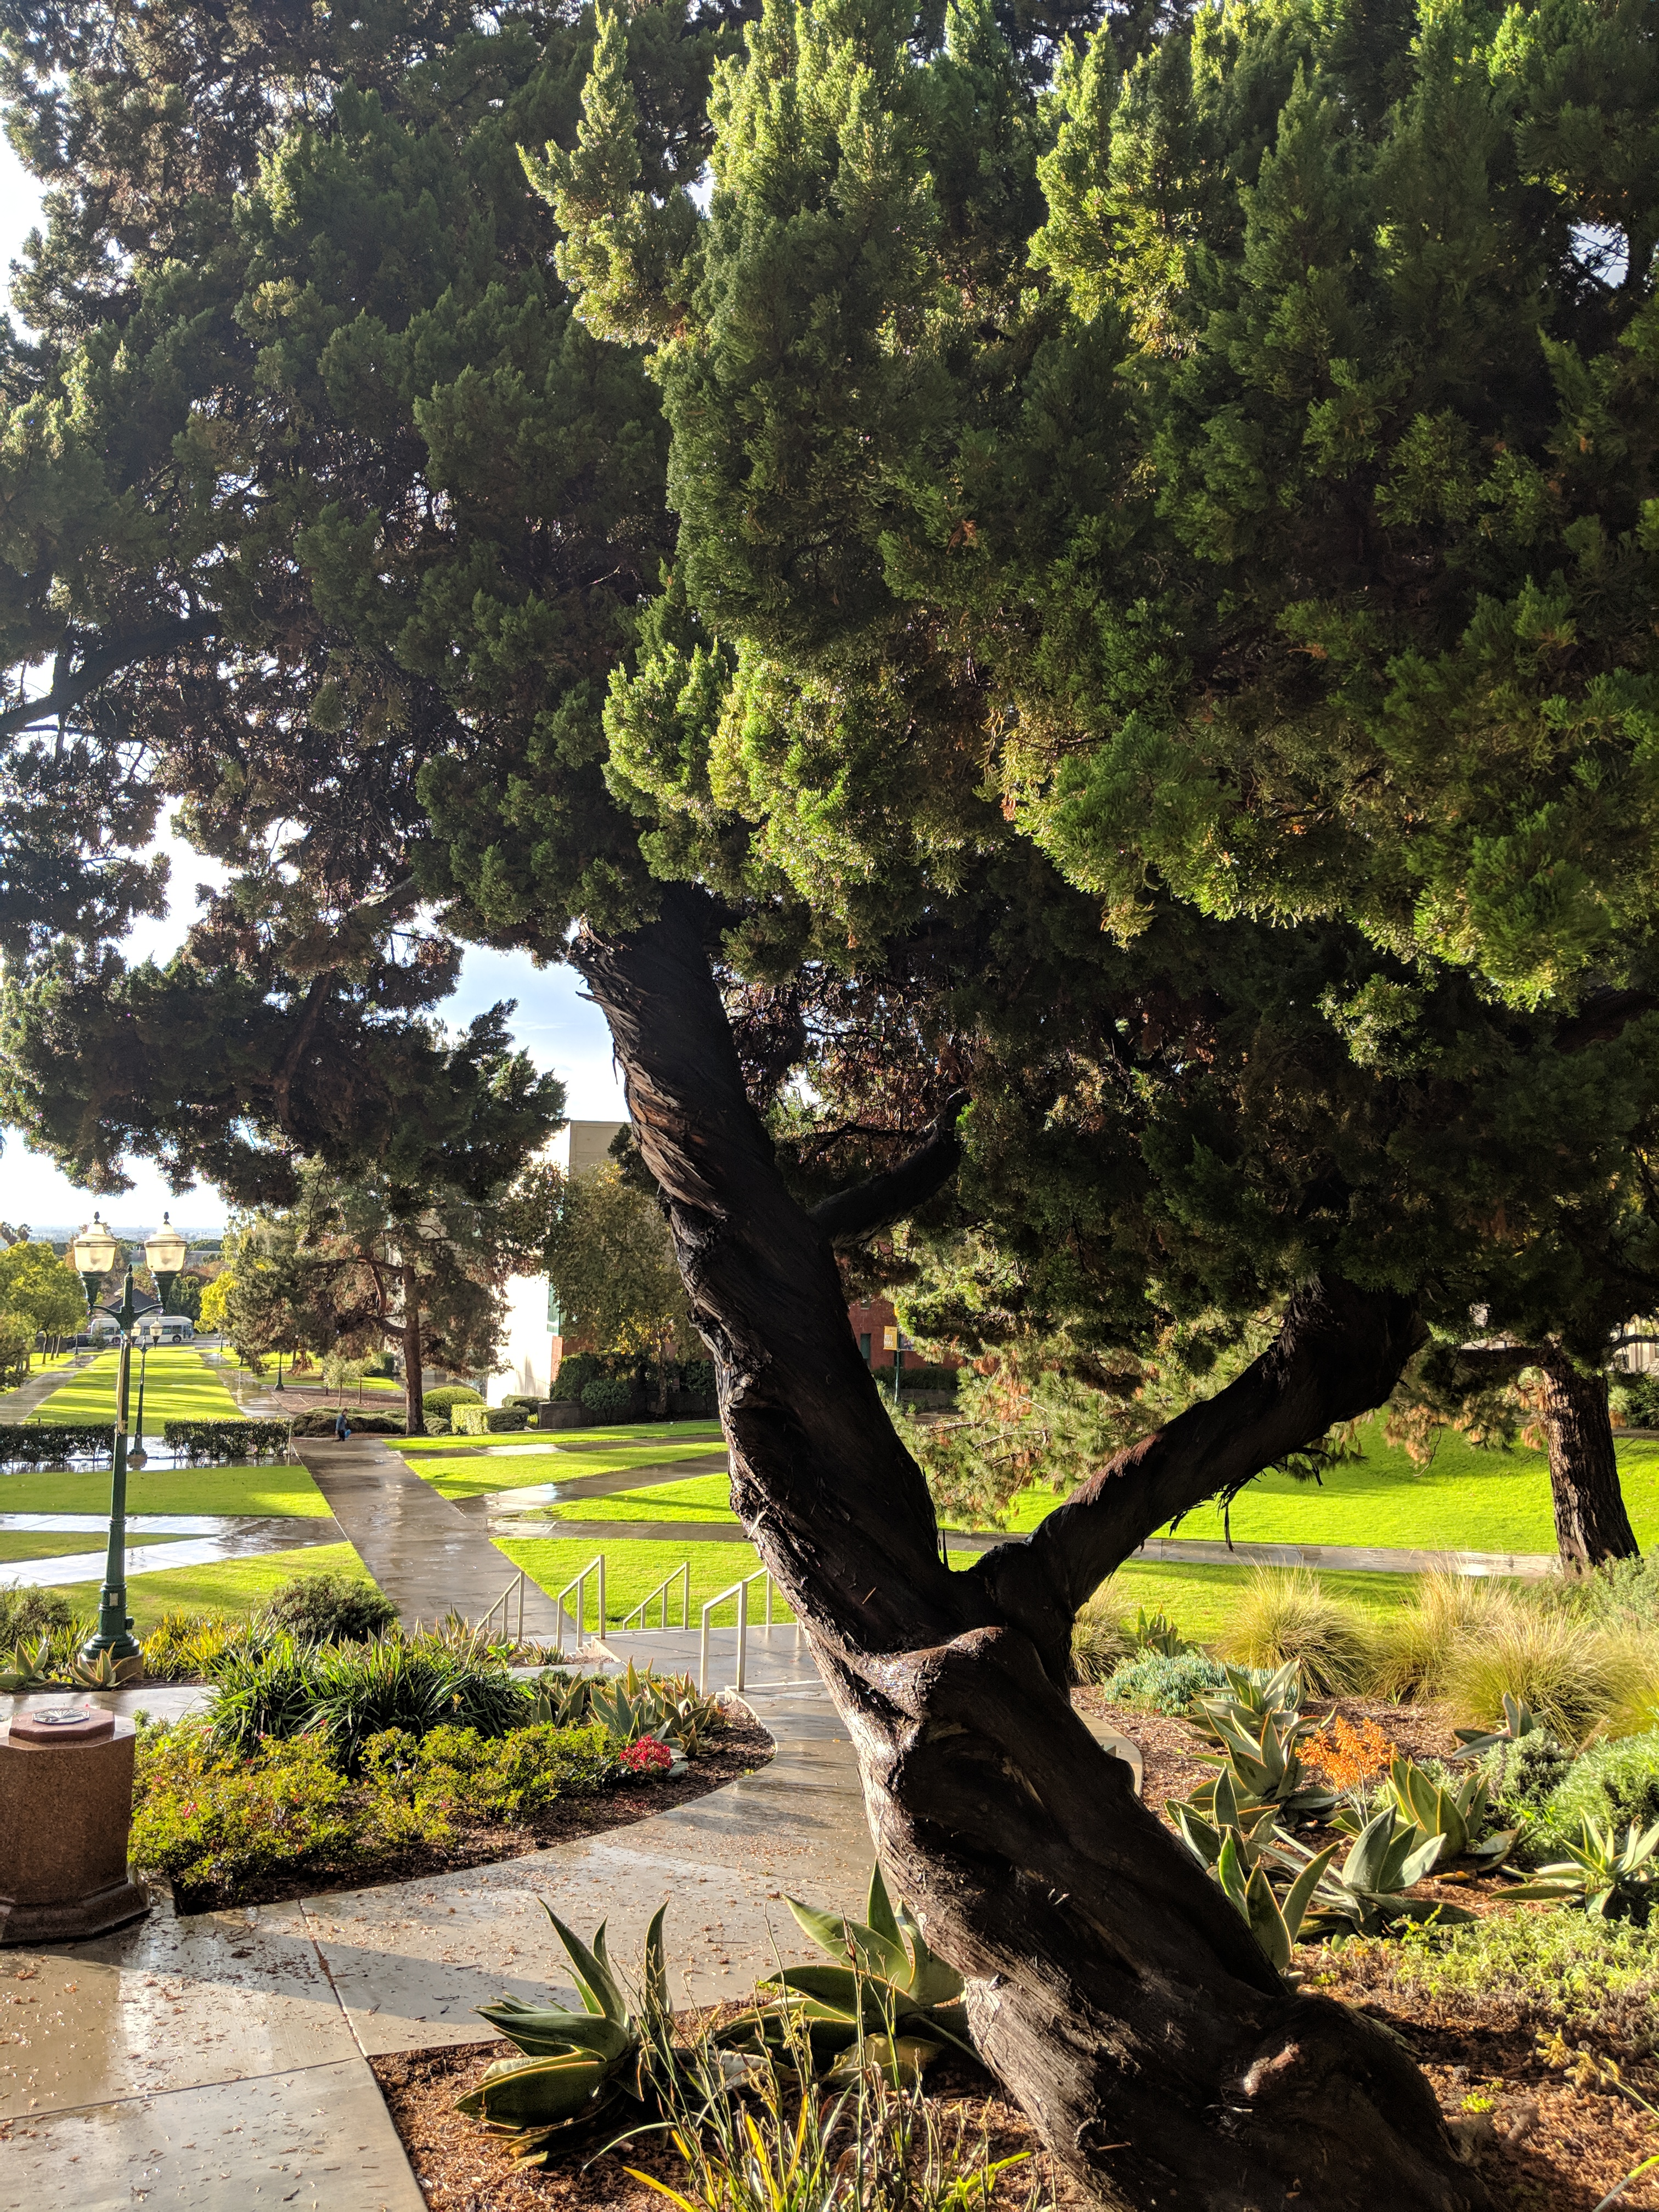
\includegraphics[width=0.4\textwidth]{tree.png}
\caption{\label{fig:tree} A person exerts a force on a rope tied to their vehicle and a tree.}
\end{figure}
\item Commercial airplanes are sometimes pushed out of the passenger loading area by a tractor. (a) An 1800 kg tractor exerts a force of $1.75 \times 10^4$ N backward on the pavement, and the system experiences forces resisting motion that total 2400 N. If the acceleration is 0.12 m s$^{-2}$, what is the mass of the airplane?  \textit{Hint: think of the tractor and airplane as one system.} \\ \vspace{3cm}
\end{enumerate}

\section{Chapter 5: Further Applications of Newton's Laws}

\begin{enumerate}
\item 
\begin{figure}
\centering
\includegraphics[width=0.3\textwidth]{friction2.png}
\caption{\label{fig:fric} A table of friction coefficients.}
\end{figure} 
Suppose a 60 kg snowboarder is on top of a waxed wood snowboard, and is sliding across snow.  (a) If her initial speed is 12 m/s, what is her deceleration due to friction?  (b) When will she stop?  (c) How far will she travel? \\ \vspace{2.0cm}
\item The snowboarder from the previous problem drops down a slope with an incline angle of 10 degrees.  (a) Draw a free body diagram below (include friction).  (b) What is her acceleration?  (c) Suppose the snowboarder starts with no initial velocity.  If the hill is 50 meters long, what will be her final speed at the bottom? \\ \vspace{2.0cm}
\item Suppose a 65 kg snowboarder is on top of a waxed wood snowboard, and is sliding across snow.  (a) Draw a free-body diagram accounting for friction, drag, gravity, and the normal force.  (a) Suppose he is moving at 10 m/s, his drag coefficient is $C = 0.9$, and he has an area of $1.2$ m$^2$.  At the moment he is moving at 10 m/s, what is his deceleration, accounting for both friction and drag?  The density of air is 1.225 kg m$^{-3}$. \\ \vspace{2.5cm}
\item Suppose a micro-organism of radius 100 $\mu$m ($100 \times 10^{-6}$ m) and density 1000 kg m$^{-3}$ is located at the top of a pond that is 3 meters deep.  (a) Draw a free-body diagram involving the Stoke's Law drag force, and gravity.  (b) What is the terminal velocity?  (c) Assuming it travels at this velocity, how long does it take to reach the bottom of the pond? \\ \vspace{2cm}
\item A 10 m steel beam with cross-sectional area $0.125$ m$^2$ has a Young's modulus of $200 \times 10^9$ N m$^{-2}$.  If it holds a mass $m$ on top of it, and it is compressed by 1 mm, what is $m$ in kg?
\end{enumerate}

\end{document}